\chapter{Tools}
\label{chapter:tools}


\section{Web Development Languages}

\begin{table}[ht]
\centering
\caption{Ranking among the most used languages on GitHub \parencite{stateOfTheOctoverse23}}
\label{tab:githubMostUsedLanguageRanking23}
\begin{tabular}[t]{|l|r|}
\toprule
Language & Rank\\
\midrule
JavaScript & 1\\
Python & 2\\
TypeScript & 3\\
C++ & 6\\
\bottomrule
\end{tabular}
\end{table}


\subsection{JavaScript}

A scripting language created by Brendan Eich in 1995 as part of the release of the \emph{Netscape 2} browser \parencite{javascriptRelease}, then was officially standardised by the Swiss standards body \emph{Ecma} in 1997 as \emph{ECMA-262} or \emph{ECMAScript}, as it is known today. This standard later was the basis for \emph{JScript} by \emph{Microsoft} and \emph{ActionScript} as part of \emph{Macromedia Flash}. The version currently being supported by all browsers (except Internet Explorer 11) is \ac{ES6} \parencite{javascriptHistory}.

\ac{JS} is an object-oriented, weakly-typed programming language that applies multiple programming paradigms. It is primarily used in the browser to add extra functionality to web pages. The underlying \emph{ECMAScript} standard does not define any input or output methods, which means that this is provided by the specific environment it is being used in (e.g. desktop or mobile browsers).

\subsection{TypeScript}

\ac{TS} was released by Microsoft in 2012 \textquote[\cite{typescriptRelease}]{to accommodate an increasing number of developers who are interested in using JavaScript to build large-scale Web applications to run in a browser rather than on the desktop.} It complies with the underlying Ecma scripting standard and is designed as a superset of \ac{JS}, adding static typing. It uses a compiler to generate regular \ac{JS} code.


\section{Native Application Development}

\subsection{Node JS}

Released initially by developer Ryan Dahl in 2009, a server-side \ac{JS} environment, Node.js runs standard ECMAScript in Google's V8 engine, allowing multithreading and native code integration. Its development was sponsored by the company Joyent after some dissatisfaction in the community about Joyent's stewardship and a fork of Node.js called io.js. These differences were eventually resolved, and everything was merged under the umbrella of the OpenJS Foundation. 

Node.js uses the \ac{NPM} to package code as modules, which can be used as dependencies. These modules can also integrate native C++ code, enabling bindings to most open-source libraries in the Linux ecosystem. It can be used to develop \ac{API}s or other server-side applications and support local web development processes like preprocessing, packaging, and deployment. 

\subsection{Python}

Guido van Rossum created the Python programming language in 1990 \parencite{pythonHistory}. It is a multi-paradigm language that is both dynamically and strongly typed \parencite{pythonTyping}. It relies heavily on indentation and whitespace to structure the code.

The language uses a standard library, and the surrounding ecosystem of available modules and applications based on Python makes it a good choice for data processing and science.

There is a native code interface that allows extending Python with bindings to native code, like with Node.js.

\subsection{C/C++}

C++ originated as an extension to C in 1985. It is a multi-paradigm, statically typed and object-oriented programming language.

It can be used to develop code for embedded platforms like Arduino, extend both Node.js and Python and, more generally, provide direct interaction with the operating system and its APIs.


\section{Frontend Frameworks and Libraries}

There is a wide range of available \ac{JS} frameworks to build dynamic frontends for \ac{SPA}s and \ac{PWA}s. The three libraries currently dominating the landscape are \emph{React}, developed by \emph{Facebook} in 2013, and \emph{Vue.js}, created by Evan You in 2014. These libraries can be used with frameworks to offer complete routing and state management solutions. Another popular framework is \emph{Angular}, initially released by \emph{Google} in 2010 and re-released in 2016.

\begin{figure}[h]
    \centering
    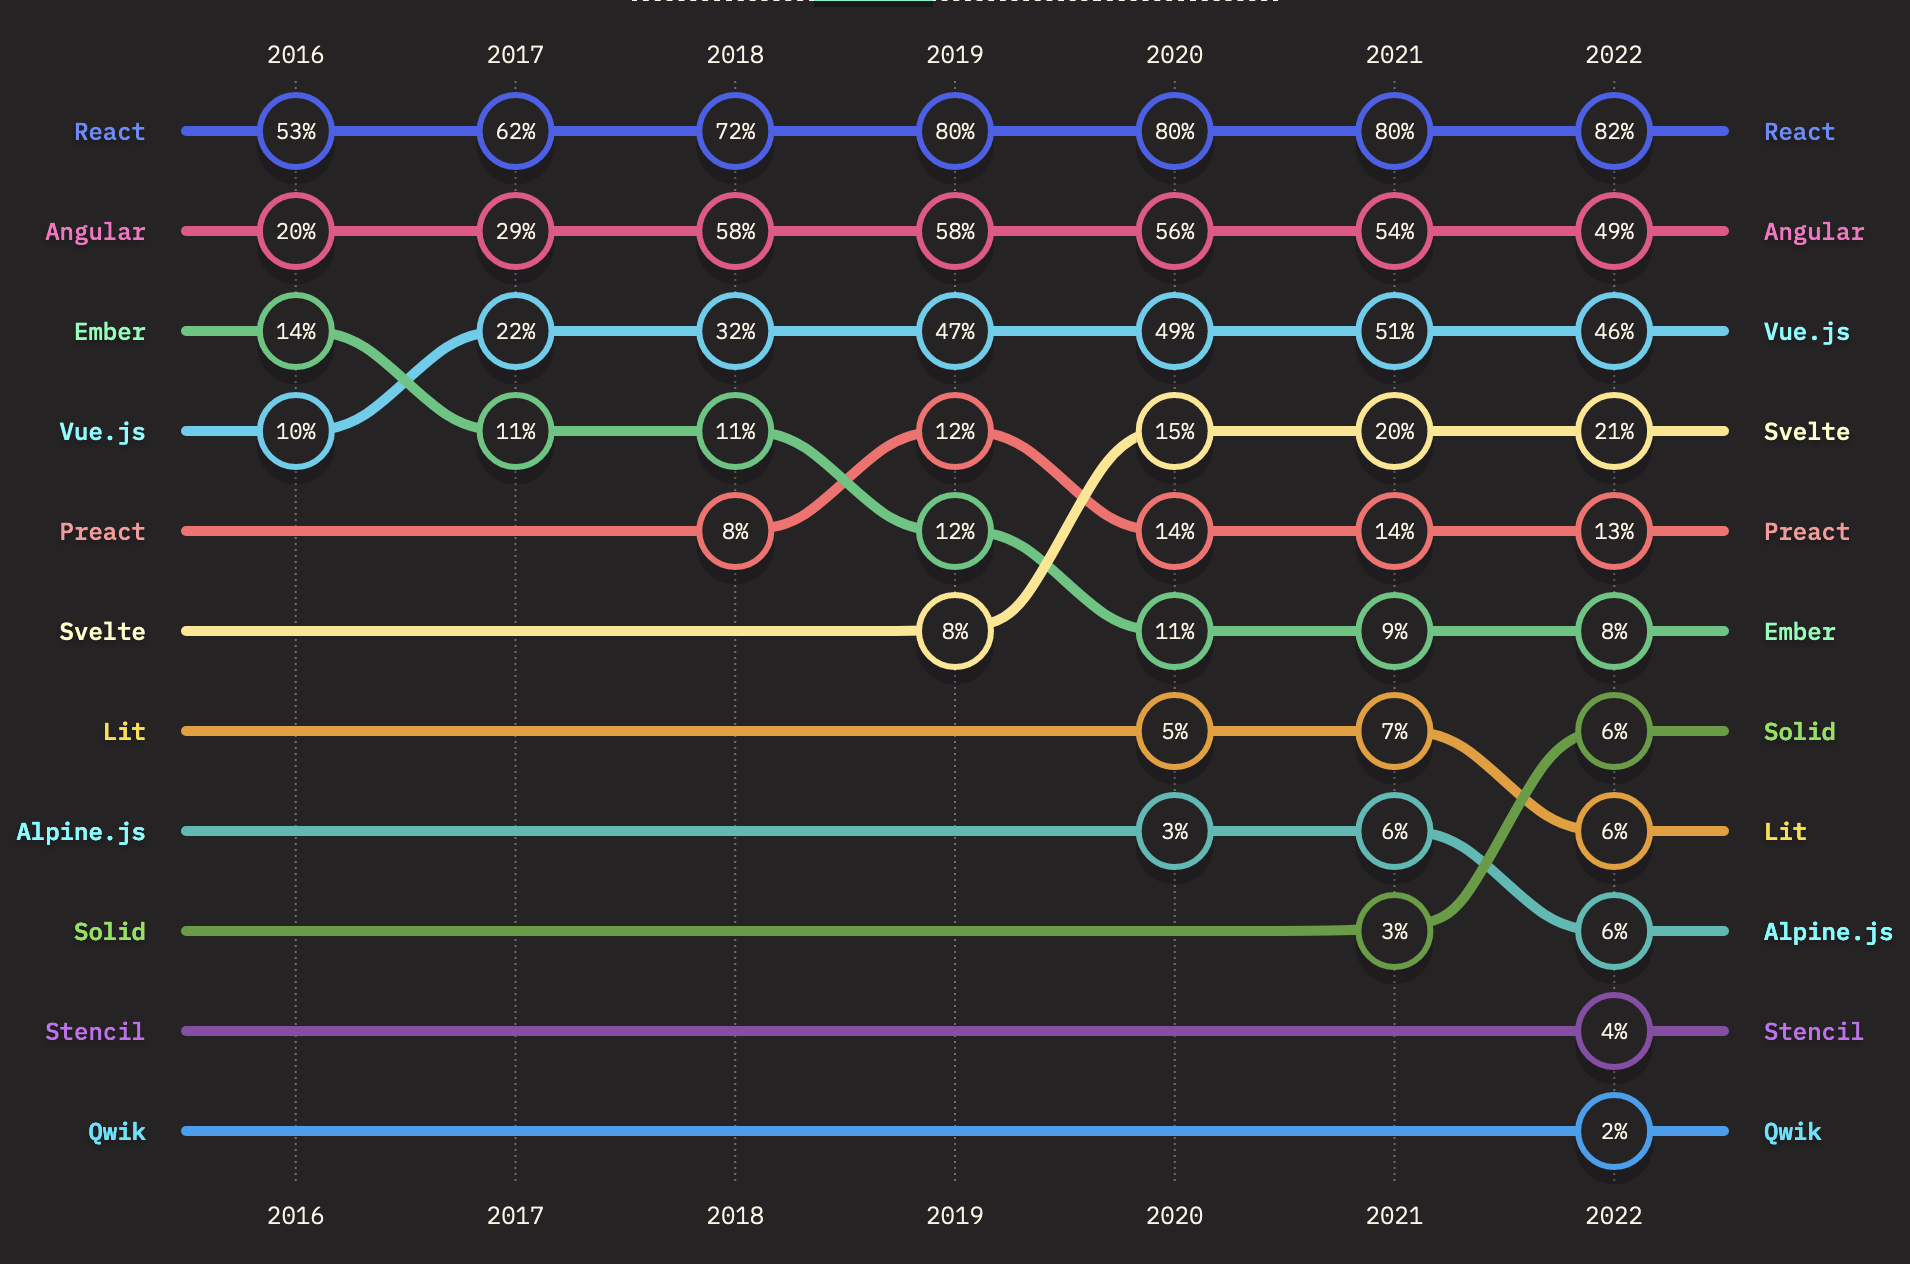
\includegraphics[scale=0.4]{04_Artefakte/01_Abbildungen/stateofjs-usage-frontend-frameworks-2022}
    \caption[{Most used frontend frameworks in 2022}]{State of JS: Most used frontend frameworks in 2022\protect\footnotemark}
    \label{fig:mostUsedFrameworks}
\end{figure}
\footnotetext{\cite{mostUsedFrontendFrameworks22}}

\subsection{React}

\emph{React} (\url{https://react.dev/}), developed by \emph{Facebook} and maintained by its successor \emph{Meta}, has become the most widely used tool for building \ac{SPA}s and is steadily leading the rankings for most used frontend frameworks both in the \emph{StackOverflow} \parencite{stackOverflowPollWebFrameworks23} and the \emph{State Of JS} \parencite{mostUsedFrontendFrameworks22} polls. By definition, it is not a framework but a \ac{UI} library that builds on other extensions to support state management, routing and deployment functionality. Although it is not a framework itself, there are existing frameworks like \emph{Next.js} (\url{https://nextjs.org/}) for the web and \emph{ReactNative} (\url{https://reactnative.dev/}) for building mobile apps using native functionality. React makes use of \ac{JSX}, which allows directly mixing inline \ac{HTML} with the \ac{JS} or \ac{TS} code structure.

\subsection{Vue.js}

\emph{Vue.js} (\url{https://vuejs.org/}) was developed by Evan You and is maintained by an international team of individuals. It had a relatively marginal presence in the US and Europe in the first years after its inception. This can be partially attributed to its origin in China, as most of its supporting modules were localised in Chinese. Over the years, it grew in popularity and received much more international support, eventually overcoming the language barrier. Unlike \emph{React}, it is billed as a "progressive framework" that provides fundamental functionality for building reactive components but also accommodates more complex use-cases \parencite{vueProgressiveFramework}. \emph{Vue.js} builds on standard \ac{JS} or \ac{TS}, \ac{HTML} and \ac{CSS} to build components, recommending a simple template mechanism mixed with reactive substitutions. However, it also supports using \ac{JSX} for specifying inline \ac{HTML} within \ac{JS}. As with \emph{React}, there are extensions and frameworks like \emph{Quasar} (\url{https://quasar.dev/}) and \emph{Nuxt} (\url{https://nuxt.com/}) that enable even more sophisticated workflows for application development and deployment.

\subsection{Angular}

\emph{Angular} was initially released by \emph{Google} in 2010 as \emph{AngularJS}  and officially discontinued in 2022 (\url{https://angularjs.org/}). A completely overhauled and currently used version 2 was released in 2016 and maintained by \emph{Google}. It is different from \emph{React} and \emph{Vue.js} in that it is a complete framework that contains everything required to build and deploy an application, and it explicitly recommends \ac{TS} as a programming language. The framework is also less flexible in that it is opinionated and has its own set of best practices baked into the framework's structure.




\section{Backend Libraries}

\subsection{Express}

The Express JS framework provides the basic functionality to create web servers, including routing and middleware functionality. TJ Holowaychuk developed and sold it to StrongLoop, which IBM subsequently acquired. It is currently under the stewardship of the OpenJS Foundation.

Express has become the de facto standard for building web services in JS, leading the ranking in the State of JS survey \parencite{mostUsedBackendFrameworks22}. Although it contains the necessary parts to make a web service, it does not enforce a specific architecture, which can be problematic for maintaining a robust application structure. For developers who prefer a more explicit structure, various other frameworks are built on top of it that add more opinionated structures or extensions.

\subsection{Koa}

Billed as a successor to Express, Koa is developed by the team behind Express. It aims to provide a more robust and minimalistic iteration of the middleware-based architecture of Express. Like Express, it allows for building a service from scratch in free form but is also the basis for other, more explicitly structured frameworks.


\section{Backend Frameworks}

Other frameworks and a more stringent and structured application structure might be more desirable for complex applications. There are numerous \ac{JS} frameworks, some based on Express or Koa, and others provide their own basis for routing. To review all possible options is beyond the scope of this study. In the following, three frameworks are selected for their specific nature related to popularity and stability, with an explicit focus on real-time applications.

\begin{table}[ht]
\centering
\caption{State of JS survey: Most used backend frameworks \parencite{mostUsedBackendFrameworks22}}
\label{tab:backendFrameworksRanking}
\begin{tabular}[t]{lcc}
\toprule
Framework & \% of question respondents\\
\midrule
Nest & 30.2\\
Feathers & 8.8\\
Meteor & 2.7\\
\bottomrule
\end{tabular}
\end{table}


\subsection{Nest JS}

Nest JS is a backend framework for developers who look for a more strictly opinionated and robust setup than Express, e.g. for enterprise applications. It follows a modular concept, making dependencies available to the services via injection. There are multiple database options, and transports can be HTTP and WebSockets. There are \ac{CLI} scripts that enable automatic generation of boilerplate application code, and the language used to build Nest applications is TypeScript. It ranks second among the most-used backend frameworks in the State of JS survey \parencite{mostUsedBackendFrameworks22}.

\subsection{Feathers}

This framework takes a different approach, making few assumptions about the specific application structure. It uses aspect-oriented programming and a service-centric architecture and before-, after- and around-hooks (so-called \textquote{cross-cutting concerns}) for the services that modify basic behaviour or add functionality. There are adapters for a wide range of databases and authentication methods. The framework has a dedicated concept of channels that enable real-time functionality and messaging to clients. Real-time transports are also abstracted and can be deployed using different WebSockets libraries. It also provides a \ac{CLI} to generate application code that can be written in \ac{JS} or \ac{TS}.

Feathers started as a hobby project by David Luecke and Eric Kryski in 2013 \parencite{feathersFrameworkHistory} and is currently maintained by David Luecke and a community of individual contributors. It still ranks in the lower percentages in the State of JS survey but almost doubled that percentage from the previous one in 2021 \parencite{mostUsedBackendFrameworks21}.

\subsection{Meteor}

Meteor focuses explicitly on real-time applications using WebSockets. The framework is a bit of an outlier in that its core is open-source, but other parts are proprietary code. Nonetheless, it should be mentioned because it has been around for over ten years and uses WebSockets exclusively. It was released in 2012 by a startup company, immediately received venture capital funding from Andreessen Horowitz and was eventually sold to Tiny Capital in 2019 \parencite{meteorSaleTinyCapital}.

The framework primarily uses MongoDB as a database system and initially provided its own package manager and ecosystem, build system, and template system based on Mustache. This exclusive strategy has been abandoned in favour of adopting the Node Package Manager. Still, it seems to be subject to debate regarding its ease of use versus its \textquote{growing pains} and related trouble with wide adoption \parencite{meteorDiscussionYCombinator}.



\section{Virtual and augmented reality}

\subsection{THREE.js}

This \ac{3D} graphics framework with a large community with over 1800 contributors has been around since it was publicly released by Ricardo Cabello in 2010. It features an extensive toolset for graphics generation, rendering and effects and relies on the \emph{WebGL} standard to allow performant rendering via local graphics hardware.

\subsection{A-Frame}

Based on THREE.js, this framework allows the developer to create \ac{3D} scenes by composing custom HTML elements that provide geometric primitives, lights, cameras, etc. This way, it has a low entry barrier for people coming from web development with limited scripting experience. It explicitly focuses on mixed reality applications, implements the WebXR standard and controls for various headsets and controllers.

\subsection{Resonance}

Resonance was developed by Google-based Omnitone, another Google project focusing on ambisonic spatial audio rendering. It received only one release and seems to have remained dormant since then, but it still works without breaking changes. It uses a default \ac{HRTF} to model audio spatialisation. It allows a virtual room to be created with different materials for walls, floors, and ceilings that provide different reflection types. It also offers custom sources to be defined, connected to web audio nodes, and positioned around the virtual space. It hooks into any existing audio context, thus allowing a combination with any WebAudio-compliant audio framework.

\subsection{Howler.js}

Howler is a more complete audio framework that builds on the WebAudio \ac{API} and provides easier access to audio functionality. It offers spatial audio as a plugin, but at the time of writing, only supports connecting live audio sources through a yet unmerged pull request on GitHub (see: \href{https://github.com/goldfire/howler.js/pull/1634}{https://github.com/goldfire/howler.js/pull/1634}).


\section{WebRTC}

Quite a number of software solutions for streaming media also support the WebRTC standard. However, in this case, focusing on the concept of a \ac{SFU} is essential, so the selection is reduced to the packages that explicitly focus on this type of topology.

\begin{table}[ht]
\centering
\caption{WebRTC servers ranked by stars received on GitHub}
\label{tab:githubStarsRankingWebRTC}
\begin{tabular}[t]{lcc}
\toprule
WebRTC Server & Stars & Year of initial commit\\
\midrule
Janus Gateway & 7.6k & 2014\\
LiveKit & 6.4k & 2020\\
Mediasoup & 5.7k & 2014\\
Jitsi Videobridge & 2.8k & 2013\\
\bottomrule
\end{tabular}
\end{table}


\subsection{LiveKit}

A dedicated \ac{SFU} server including \ac{SDK}s for web, native mobile and desktop and server applications in various languages. It is developed and maintained by a relatively young company, as it was publicly released in 2021 and was \textquote{started amid and in response to the pandemic} with the idea of providing \textquote{free and open infrastructure capable of connecting anyone} \parencite{livekitAbout}. While the software is free and open-source, a paid hosted service is also offered for those who want to experiment with real-time communication but don't want to set up an infrastructure. There are many examples of integration into existing frameworks, extensions for recording sessions on the server, as well as extended handling of streams.

\subsection{Mediasoup}

Mediasoup can be placed at an opposite end of the spectrum regarding high-level versus low-level frameworks. It provides a versatile collection of Node.js, Rust and C++ libraries that allow for building a custom server application from the ground up. While it takes care of the low-level \ac{RTC} functionality, it provides somewhat granular building blocks to set up the actual implementation. This allows for building entirely decentralised peer-to-peer applications as well as server-centric setups. It was developed by a small team of contributors around its leading developers, Iñaki Baz Castillo and José Luis Millán.

\section{Databases}

\subsection{MongoDB}

A document store database that is designed to hold large amounts of unstructured data. It has its own query language and features aggregation functionality that allows map/reduce and transformation operations or resolving of relations on the data before being sent to the client. Its focus on storing documents of any kind can become problematic since it can lead to inconsistent data very easily if appropriate care isn't applied in the application development (it supports schema validation, but that is not mandatory). However, this loose schematic handling can be beneficial if the application data can't be adequately modelled from the get-go and is subject to more frequent changes.

\subsection{PostgreSQL}

This very widely used database uses a table-based data topology and implements \ac{SQL} for interaction with the database and its contents. The relatively rigid database schema provides a more solid structure for data storage and retrieval but, on the other hand, requires migrations to be written to transition from one database structure version to another. This can become tedious if the data modelling process is continuously ongoing and volatile.
